\documentclass[11pt]{beamer}
\usetheme{Boadilla}
\usepackage[utf8]{inputenc}
\usepackage[czech]{babel}
\usepackage[T1]{fontenc}
\usepackage{amsmath}
\usepackage{amsfonts}
\usepackage{amssymb}
\usepackage{graphicx}
\usepackage{listings}
\author{Jan Tušil}
\title{An Executable Formal Semantics of C++}
%\setbeamercovered{transparent} 
%\setbeamertemplate{navigation symbols}{} 
%\logo{} 
\institute{FI MU} 
\date{1.2.2017} 
%\subject{} 


\lstset {
	basicstyle=\ttfamily
}

\begin{document}


% Osnova:
% Kdo jsem - Muj obor (PdS), 
% Kontext
% Cile prace
% Co se podarilo
% Dalsi kroky
% Co chci zminit:
% - kdo me vedl, s kym jsem praci konzultoval, UIUC, RV


% Koho mam v komisi? Pelanek, Strejcek, Hlineny. Vsichni trochu do tech formalnich
% metod vidi. Strejda praci cetl, tedy musim se ji snazit prodat hlavne Pelankovi a Hlinenemu.
% Nesmim se poustet do spekulaci.
% K tomu, ze jsem nasel chyby v Gcc a Clang, a nejakou nejednoznacnost ve standardu:
% to neni tim, jaky jsem borec. To se proste stava, kdyz nekdo neco formalizuje. Kdyz lidi
% pracovali na semantice JavaScriptu, take nasli chyby v interpreterech. A ted behem praci
% na formalizaci Etherea.

% K cemu je ta semantika dobra? Jak se to testuje? Mame interpreter, ktery ji pouziva.

% Dobrý den, já jsem Honza Tušil a rád bych vám představil svoji diplomovou práci, 
% ve které jsem se zabýval vytvářením spustitelné formální sémantiky pro jazyk C++.
\begin{frame}
\titlepage
\end{frame}

% TODO čítač stránek, progress bar apod. Mezislajdy mezi sekcemi.

% Během následující čtvrthodinky nejprve přiblížím kontext mojí práce,
% poté ukáži, co jsem vlastně dělal, a nakonec (shrnu?) jak to všechno dopadlo.
\begin{frame}
\tableofcontents
\end{frame}


% O mě, o C++, K framework (přepisování termů), k cemu to, RV, UIUC
% Moje osobní motivace - ověřování higlevel vlastností programů v C++ (šablony apod).

\section{Kontext}

% Moderní programovací jazyky jsou hodně mocné - a hodně složité.
% 
\begin{frame}{Jazyk C++}
\includegraphics[width=1.0\linewidth]{img/cppmap.png}
%TODO link
\end{frame}


% Nebudu zde ukazovat, jakým způsobem se K framework používá
% prakticky; kdyby vás to zajímalo, v mé práci je tomu věnována
% celá jedna kapitola.

% OT: K Framework se stále vyvíjí - některé implementační detaily
% se od odevzdání práce změnily.
\begin{frame}{K Framework}
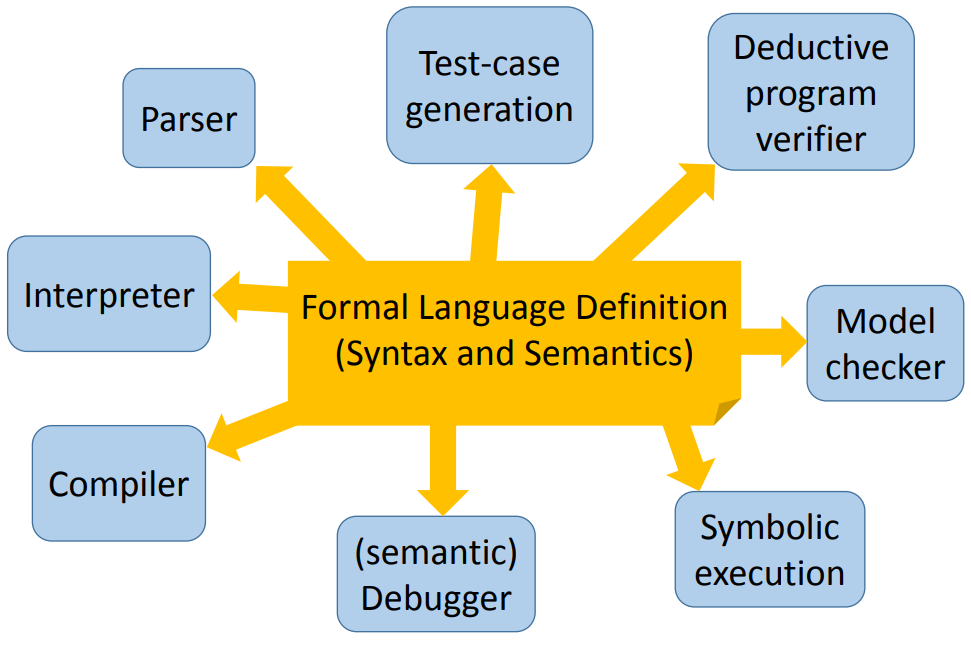
\includegraphics[width=1.0\linewidth]{img/kidea.png}
\end{frame}

% UIUC, RV
\begin{frame}{Kdo}

\end{frame}

% Jaké je současné využití.
\begin{frame}{C/C++ @ K}

\end{frame}

% Zadání, cíle, konkrétní věci, nalezené chyby apod.
\section{Obsah práce}


% Cílem mé práce bylo rozšířit stávající prototyp
% C++ sémantiky v K o dosud neimplementované vlastnosti tohoto jazyka.

% První vlastností, kterou jsem zamýšlel implementovat,
% jsou výčtové typy. V projektu sice výčtové typy byly implementovány,
% ale jen pro jazyk C. V jazyce C++ se výčtové typy chovají trošku jinak,
% navíc ve standardu C++11 (z roku 2011) přibyla nová varianta těchto typů.

% Další vlastností, kterou jsem chtěl implementovat, byla podpora vykonávání kódu
% v době překladu. Od standardu C++11 je možné označit některou z funkcí
% jako 'constexpr', což v praxi znamená, že volání takovéto funkce je možné
% vyhodnotit již v době překladu. Výpočet pak není nutné dělat za běhu,
% což může výrazně pomoci jak výkonu programu, tak čitelnosti jeho kódu.
% Výsledek výpočtu je navíc možné použít i na místech, kde jazyk vyžaduje použití konstanty.
% A ano - jazyk C++ je díky této vlastnosti turingovsky úplný už v době překladu.
% Jenže on byl turingovsky úplný již dávno předtím.

% Přestože jsem to původně neměl v úmyslu, na popud jednoho z hlavních vývojářů projektu
% jsem implementoval vlastnost, která se nazývá "nulová inializace tříd".
% Myslel jsem si, že to bude hračka, ale zabralo mi to dost dlouhou dobu.
% Jedním z důvodů byla i chyba v projektu, která se projevovala až tehdy,
% když jsem se pokoušel nulovou inicializaci naimplementovat. Chybou byl
% nedeterminismus v sémantice, který umožňoval interpretovat některé programy vícero způsoby.

% Tím se dostáváme k poslednímu bodu - opravě některých stávajících chyb.
% Projekt C++ sémantiky v K je stále v experimentální fázi,
% a tak se při práci častokrát stalo, že jsem narážil
% na nějakou chybu či nedokončenou implementaci. Opravoval jsem zejména
% ty, které mi nějak překážely.

% Ještě doplním, že z těchto čtyř bodů byly jen první dva
% součástí mého oficiální zadání.

% čas: 2min 15s
\begin{frame}{Cíle práce}
\begin{itemize}
\pause \item výčtové typy (\texttt{enum})
\pause \item vykonávání kódu v době překladu (\texttt{constexpr})
\pause \item nulová inicializace tříd
\pause \item oprava stávajících chyb v projektu
\end{itemize}
\end{frame}

% Zde budou nějaké děsivé příklady
\subsection{Intriky}

% Tady bych jenom dodal, že nalezení chyb v překladačíh
% nebo standardech programovacích jazyků není až tak moc neobvyklé,
% zvlášť v kontextu formalizace těchto jazyků - JavaScript, Ethereum.
\subsection{Chyby nalezené v jiných projektech}

% Co se povedlo, co jsem se naucil, jake jsou moje dalsi plany.

% Možná mohu říci, že práce s K frameworkem sice byla složitá v tom smyslu,
% že jsem se musel naučit hodně nových věcí, vžít se do nového programovacího paradigmatu
% apod, ale nebyla potřeba žádná hluboká matematická znalost (žádné fixpointy apod).
\section{Vyhodnocení \& co dál?}

\begin{frame}{Naplnění cílů}
\begin{itemize}
\pause \item \texttt{enum} - vše hotovo, většina je v upstream
\pause \item \texttt{constexpr} - elegantní proof of concept
\pause \item nulová inicializace - hotovo
\pause \item opravy chyb - některé přijaty do upstreamu
\end{itemize}
\end{frame}

\begin{frame}{Co dál?}
\begin{itemize}
\pause \item Vše hotové do upstreamu.
\pause \item Dokončit \texttt{constexpr}.
\pause \item Šablony, vlákna, bitová pole, fold expressions, \ldots
\pause \item Jak řešit vývoj jazyka?
\pause \item Spolupráce s RuntimeVerification inc.
\pause \item Kontrakty.
\end{itemize}
\end{frame}


\begin{frame}[fragile=singleslide]{Ochutnávka}
\begin{lstlisting}
template <typename It>
bool is_sorted(It begin, It end);

/*
 * \pre valid_range(begin, end);
 * \post is_sorted(begin, end);
 */
template <typename It>
void sort(It begin, It end);
\end{lstlisting}
\end{frame}


\begin{frame}{Kontrakty}
\begin{itemize}
\pause \item Jak jim dát sémantiku?
\pause \item Volání běžných funkcí v pre/postcondition.
\pause \item A co když mají efekty? A co když ty jsou ohraničené?
\pause \item Jak je verifikovat?
\pause \item Jak využít existující abstrakce? A vzory?
\end{itemize}
\end{frame}

% Btw v C++ sémantice stále ještě není implementován switch.
% Po otázkách - kdyby chtěli vědět něco dalšího, rád si s nima popovídám.
% Co jsem se naučil: komunikace na dálku je fuška.
% S lidma z RV a UIUC se mi spolupracovalo dobře.

\end{document}